\documentclass[10pt]{ctexbeamer}
\usepackage{bm}
\usepackage{tikz}
\usepackage{amsmath}
\usepackage{graphicx}
\newfontfamily{\dengxian}{DengXian}
\newCJKfontfamily{\fzyaoti}{FZYaoTi} %方正姚体
\newCJKfontfamily{\fzjinghong}{FZZJ-JHTJW} %方正字迹-惊鸿体
\newCJKfontfamily{\dqheiti}{Hiragino Sans GB} %冬青黑体
\newCJKfontfamily{\fandolhei}{FandolHei}

% \usetheme[color blocks]{Verona}% 使用Verona主题
% \usetheme[color blocks, red]{Verona}% 使用Verona主题, red theme
% \usetheme[color blocks, gray]{Verona}% 使用Verona主题, grey theme
\usefonttheme[onlymath]{serif}% 数学公式字体设置
\author{Norsesun}
\date{最后更新:\today}
\logo{
\includegraphics[height=1.2cm]{../../../Pngtree owl double exposure.png}}

\definecolor{airforceblue}{rgb}{.36,.54,.66}



\newcommand{\bmc}[1]{$\bm{#1}$}%定义一个新命令,行内数学模式的粗体,使幻灯片上的公式更清楚
\newcommand{\bmcc}[1]{
        \begin{displaymath}
            \bm{#1}
        \end{displaymath}
    }%定义一个新命令,行间数学模式的粗体,使幻灯片上的公式更清楚
\newcommand{\makecenter}[1]{\vspace{0.5em}\centering \parbox{.6\textwidth}{#1}}%定义一个新命令,居中排布一段话
\newenvironment{Mathbreakcenter}[1][1mm]{
        \par
        \vspace{#1} 
        \centering

    }{
        \par
        \vspace{2mm}
    }
\newcommand{\myblock}[3][1-]{
    \centering
    \begin{minipage}{.6\textwidth}
        \begin{block}<#1>{#2}%
            \centering%
            #3
        \end{block}
    \end{minipage}  
    } %定义一个新命令,居中排布一个block

    \newcommand{\myalertblock}[3][1-]{
        \centering
        \begin{minipage}{.6\textwidth}
            \begin{alertblock}<#1>{#2}%
                \centering%
                #3
            \end{alertblock}
        \end{minipage}  
        } %定义一个新命令,居中排布一个alertblock
\newcommand{\cleave}[2]{
    \hbox to #1{} #2 \hbox to #1{}
}
% \newcommand{\annmark}[1]{%
%     \textcolor{red}{$\bm\langle$#1$\bm\rangle$}%
% }%

% \newcommand{\ann}[1]{%
%     \begin{tikzpicture}[remember picture, baseline=-0.75ex]%
%         \node[coordinate] (inText) {};%
%     \end{tikzpicture}%
%     \marginpar{%
%         \renewcommand{\baselinestretch}{1.0}%
%         \begin{tikzpicture}[remember picture]%
%             \definecolor{orange}{rgb}{1,0.5,0}%
%             \draw node[fill=red!20,rounded corners,text width=\marginparwidth] (inNote){\footnotesize#1};%
%     \end{tikzpicture}%
%     }%
%     \begin{tikzpicture}[remember picture, overlay]%
%         \draw[draw = orange, thick]
%             ([yshift=-0.2cm] inText)
%                 -| ([xshift=-0.2cm] inNote.west)
%                 -| (inNote.west);%
%     \end{tikzpicture}%
% }%

% \setlength{\marginparwidth}{2.5cm}
% \renewcommand{\baselinestretch}{1.3}

\newenvironment{mathsalvation}[2][{解:}]{
    \begin{center}{}
        \begin{minipage}[t]{.05\textwidth}
            \vspace{0pt}
            {\color{#2}{#1}} \quad 
        \end{minipage}
        \begin{minipage}[t]{.7\textwidth}
            \vspace{0pt}
            % \fzyaoti
            % \dengxian
            % \fzjinghong
            % \dqheiti
            \fandolhei
}{
    \end{minipage}
    \end{center}
}

\usepackage{smartdiagram}
\usepackage{bm}

\title{整式的加减}
\subtitle{Addition and Subtraction of Integral Expression}

\begin{document}
    \frame{\titlepage}

    \begin{frame}{回顾}{关于整式的加减运算, 我们已经学习过的知识}
        \begin{figure}
            \centering
            \smartdiagram[descriptive diagram]{
            {合并同类项, {怎么合并同类项?}},
            {去括号, {如何将多项式中的括号去掉?}},
        }
        \end{figure}
        

        我们可以利用\textbf{合并同类项}和\textbf{去括号}的法则进行整式的加减运算。
    \end{frame}

    \begin{frame}{例题}{Math and Success Add Up}
        \begin{block}{}
        求多项式 $3x^2+5x$ 与多项式 $-6x^2+2x-3$ 的和与差。
        \end{block}
    \end{frame}

    \begin{frame}{例题2}{Math builds your brain.}
        \begin{block}{}
        \textbf{先化简,再求值:} \\
        $5xy-(4x^2+2xy)-2(2.5xy+10)$ , 其中 $x=1, y=-2$.
        \end{block}
    \end{frame}

    \begin{frame}{整式加减法的一般步骤}{Multiply your success!}
        \begin{figure}
            \centering
            \smartdiagramset{back arrow disabled=true}
            \smartdiagram[flow diagram:horizontal]{
                有括号的先去括号, 
                合并同类项
            }
        \end{figure}
        
    \end{frame}

    \begin{frame}{例题3}{根据题意列出代数式再化简求值}
        如图,正方形的边长为 $x$, 用整式表示图中绿色部分的面积,并计算
        当 $x=4m$ 时绿色部分的面积。
        \begin{figure}
            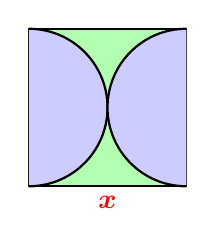
\begin{tikzpicture}
                \filldraw [thick, fill=green!30] (0, 0)  -- 
                node [color=red, pos=0.5, below, sloped]{$\bm{x}$}
                     (2, 0) -- 
                    (2, 2) -- (0, 2)--
                     cycle;
                \filldraw [thick, fill=blue!20] (0, 0) arc (-90:90:1);
                \filldraw [thick, fill=blue!20](2, 2) arc (90:270:1);
            \end{tikzpicture}
        \end{figure}
    \end{frame}
\end{document}